

% Chapter Introduction
The researcher followed different methods and 
steps to conduct this study. The data gathering
procedures, experimental design, methods and steps 
and the statistical treatment of data are also 
included in this chapter.

% Research Design 
\section{Research Design}
The research design used in this study is \emph{exploratory research}.


This design is usually used in Machine Learning researches. 

\section{Locale and Population of the Study}
The study is conducted at the comfort of the researcher's residence. 


\section{Data Gathering Instrument}
Data is the most important part of any type of Machine Learning Research. 
Since this research focuses on the feasibility of using a trained 
Convolutional Neural Network embedded in Smartphone Application to diagnose 
various plant diseases from an image of plant leaves, a plethora of 
healthy and infected plant leaf images were required to conduct this study. 

The researcher is in debt for the following datasets which were made publicly 
available. 

\begin{enumerate}
    \item \textbf{Plant Village Dataset}  \\ 
        - The PlantVillage dataset consists of $54303$ healthy and unhealthy leaf 
         images divided into $38$ categories by species and disease. 
    
         \begin{figure}[h!]
            \centering 
            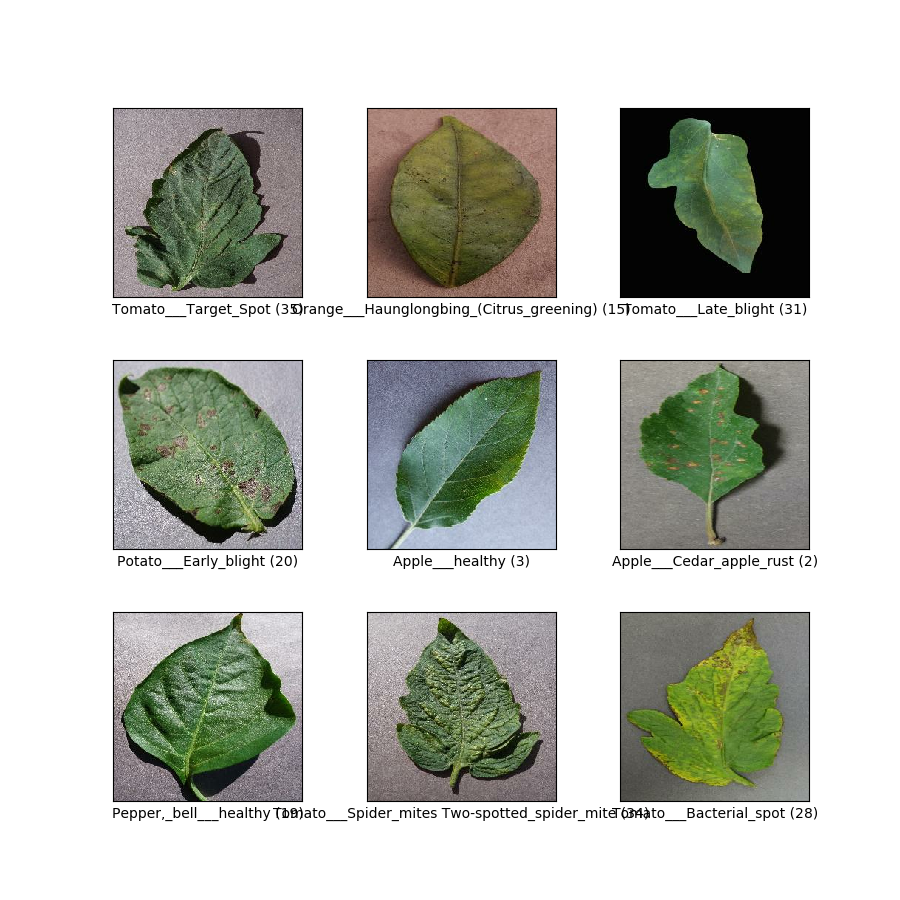
\includegraphics[scale=0.6]{plant-village-examples.png}
            \caption{Example of images in the Plant Village Dataset}
         \end{figure}


    \item \textbf{Citrus Dataset} \\ 
        - The dataset contains $759$ images of healthy and unhealthy images for both Citrus fruits and
         leaves collectively. Each image contains $256 \times 256$ dimensions with $72$ dpi resolution.  \\ 

         \begin{figure}[h!]
            \centering 
            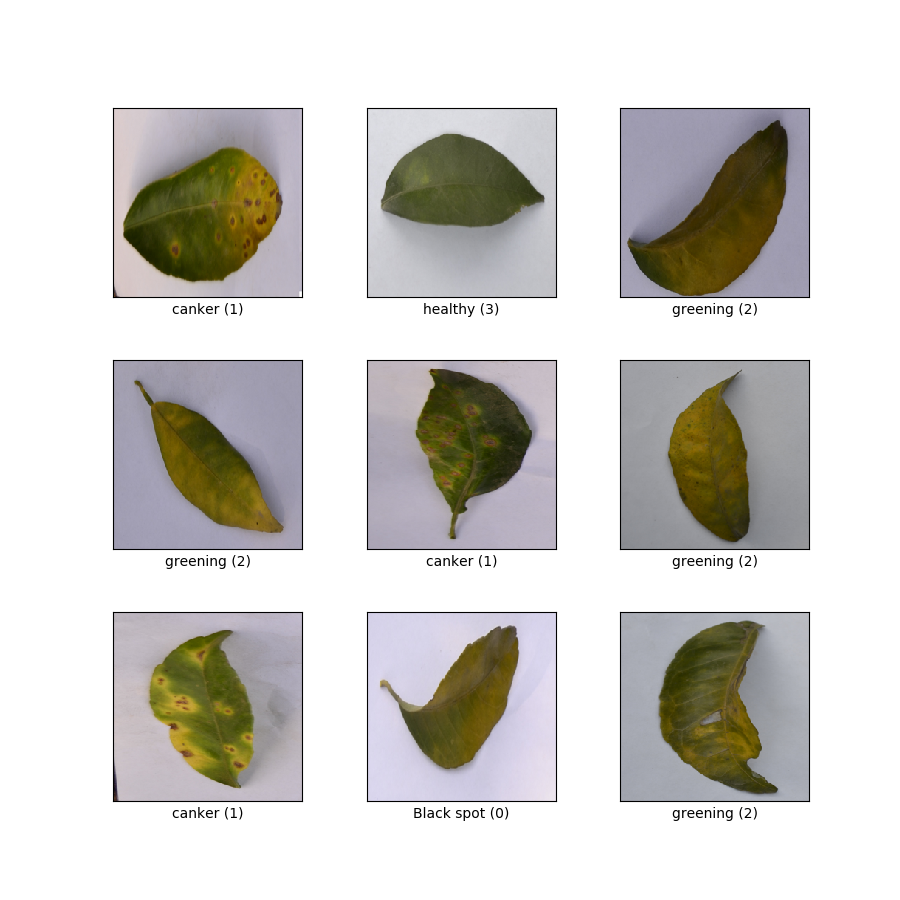
\includegraphics[scale=0.6]{citrus-leaves-examples.png}
            \caption{Example of images in the Citrus Leaves Dataset}
         \end{figure}

    % ! Temporary
    % \item \textbf{Field Images of Maize Annotated with Disease Symptoms} \\
    %     - This dataset consists of $18,222$ images annotated with 
    %     $105,705$ Northern Leaf Blight lesions.

\end{enumerate}

\section{Data Gathering Procedure}
In gathering the data required to conduct the study, the 
researcher downloaded the 


\section{Statistical Treatment}


% TODO 1. Link to the datasets